\phantom{Th}
Diagramy UML zwane również Unified Modeling Language umożliwiają graficzne przedstawienie logiki relacji, czy procesu \cite{diagram}. Są to standardy graficzne używane w inżynierii oprogramowania do modelowania struktury i zachowania systemów informatycznych. Umożliwiają one lepsze zrozumienie architektury systemu oraz pomagają w procesie projektowania i dokumentowania. Poniżej zostały przedstawione diagramy kolekcji występujących w bazie danych Firebase wykorzystywanych w aplikacji ZodiaCal.

\section{Diagram bazy danych}

\begin{figure}[h]
	\centering
	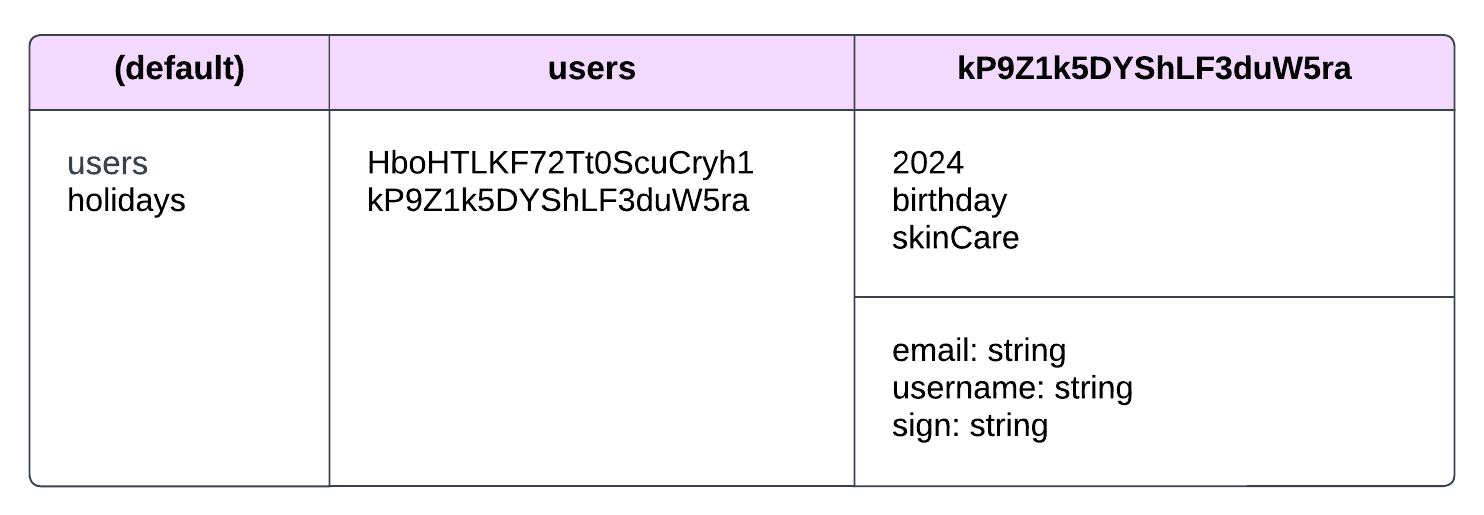
\includegraphics[width=1\linewidth]{images/model_danych/user}
	\caption{Diagram kolekcji user}
	\label{fig:user}
\end{figure}

Diagram kolekcji user (Tab. \ref{fig:user}) zawiera informację o zalogowanym użytkowniku. Każdy user posiada swój własny unikalny User UID. Podstawowe dane użytkownika to obowiązkowe pola email i user name oraz opcjonalne pole sign. Podczas korzystania z aplikacji w bazie danych tworzą się kolekcje takie jak obecny rok, w którym przechowywane są wszystkie informacje potrzebne do zarządzania kalendarzem, kolekcja birthday, w której użytkownik przechowuje daty urodzin swoich bliskich oraz kolekcję skinCare przechowujące treści dotyczące pielęgnacji cery.

\newpage

\begin{figure}[h]
	\centering
	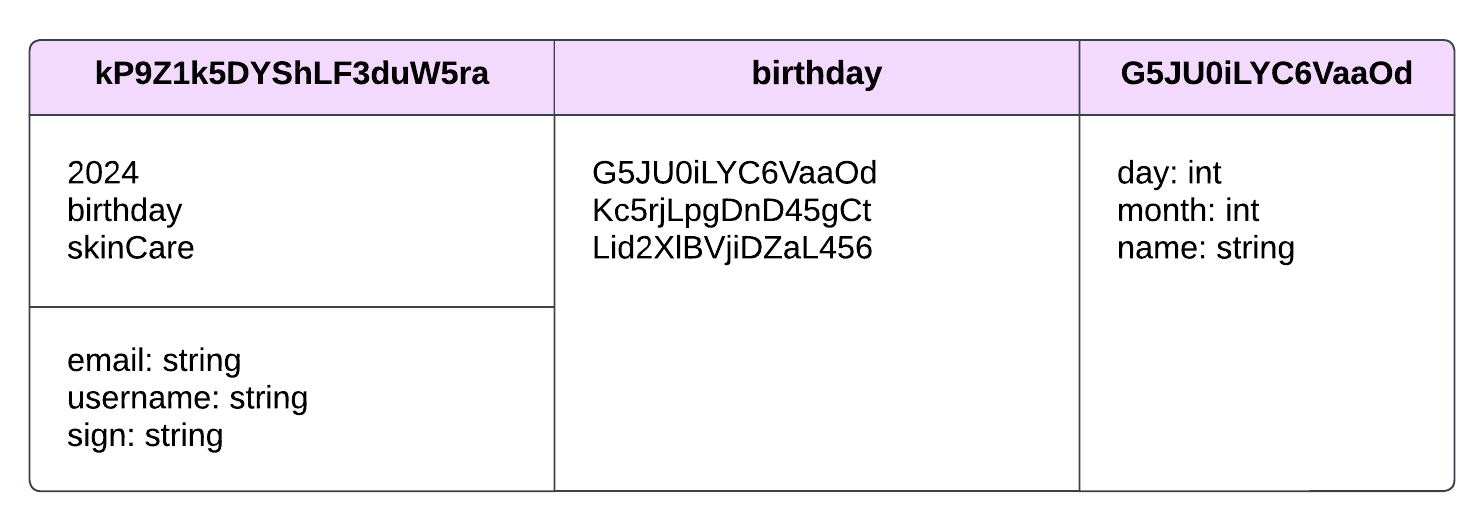
\includegraphics[width=1\linewidth]{images/model_danych/birthday}
	\caption{Diagram kolekcji birthday}
	\label{fig:birthday}
\end{figure}

Kolekcja birthday (Tab. \ref{fig:birthday}) przedstawia listę dat urodzin różnych osób. Posiada dwa pola typu int tzn. day oraz month i jedno pole typu string name, które wskazuje na imię jubilata.

\begin{figure}[h]
	\centering
	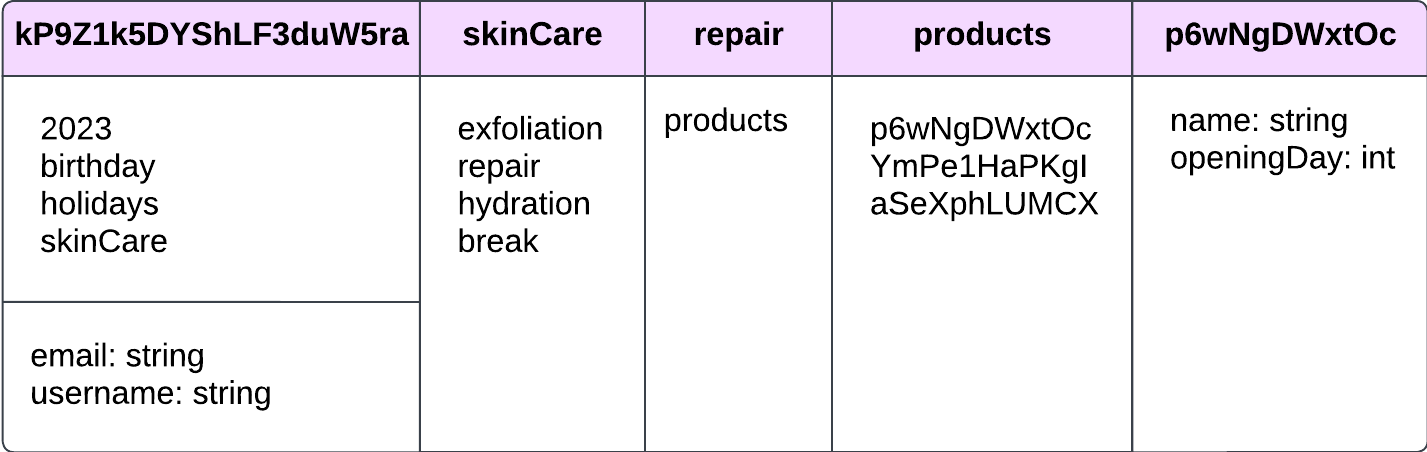
\includegraphics[width=1\linewidth]{images/model_danych/skinCare}
	\caption{Diagram kolekcji skinCare}
	\label{fig:skinCare}
\end{figure}

W tabeli o nazwie "skinCare" (Tab. \ref{fig:skinCare}), znajduje się zbiór informacji dotyczących pielęgnacji cery. W ZodiaCal zostały wyróżnione 4 rodzaje pielęgnacji: złuszczanie, odbudowa, nawilżanie oraz przerwa. Każda kolekcja danego typu pielęgnacji posiada swoje własne produkty. Produkty natomiast zawierają informację o nazwie produktu, nazwie marki oraz terminie ważności kosmetyku. Użytkownik wybiera produkty do pielęgnacji z zewnętrznego API, a następnie są one przekazywane do Firebase.

\begin{figure}[h]
	\centering
	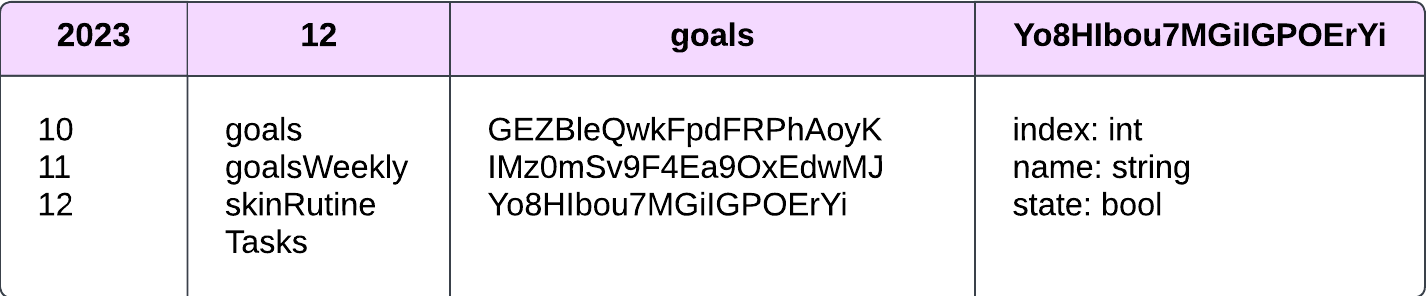
\includegraphics[width=1\linewidth]{images/model_danych/goals}
	\caption{Diagram kolekcji goals}
	\label{fig:goals}
\end{figure}

Kolekcja goals (Tab. \ref{fig:goals}) jest zagnieżdżona kolejno w kolekcji reprezentujący bieżący rok następnie bieżący miesiąc. W kolekcji odzwierciedlającej bieżący miesiąc znajdują się kolekcje dotyczące celi na dany miesiąc oraz tydzień, rutyny pielęgnacyjnej oraz zadań. Każdy cel ma swój unikalny ID, pole typu int przechowujące numer indexu, pole typu string name przedstawiające cel oraz pole typu bool state, które wskazuje czy cel został osiągnięty, czy nie.

\begin{figure}[h]
	\centering
	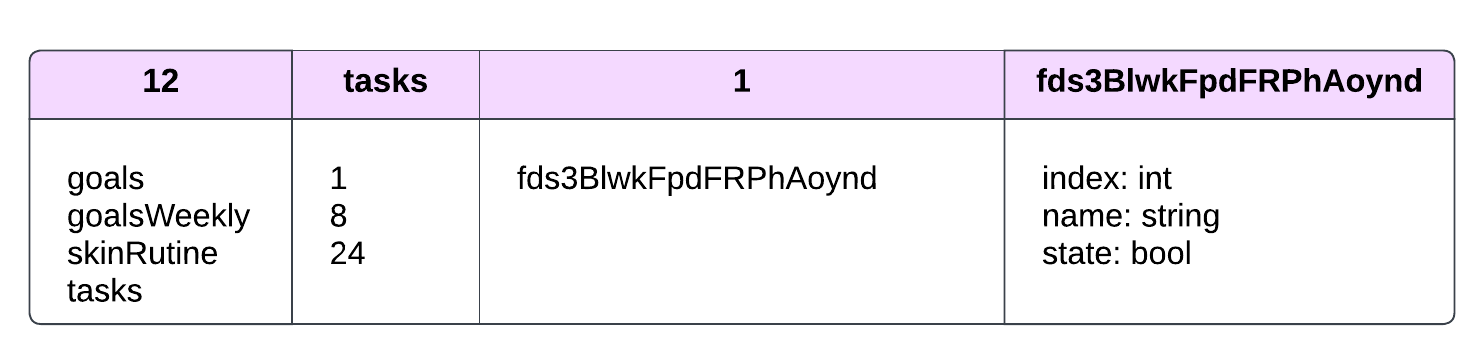
\includegraphics[width=1\linewidth]{images/model_danych/tasks}
	\caption{Diagram kolekcji tasks}
	\label{fig:tasks}
\end{figure}

Podobnie jak w przypadku kolekcji goals, tabela zatytułowana tasks (Tab. \ref{fig:tasks}) również jest zagnieżdżona w bieżącym roku oraz miesiącu. W tej kolekcji są tworzone kolejne kolekcje ilustrujące dni w danym miesiącu. Wszystkie zadania są przypisane do swoich unikalnych identyfikatorów, posiadają pola typu int, w których przechowywane są numery indeksów, pola typu string oznaczone jako "name" zawierające opis zadania, a także pola typu bool oznaczone jako "state", wskazujące na stan zadania.

\section{Diagram UML komponentów}

\begin{figure}[h]
	\centering
	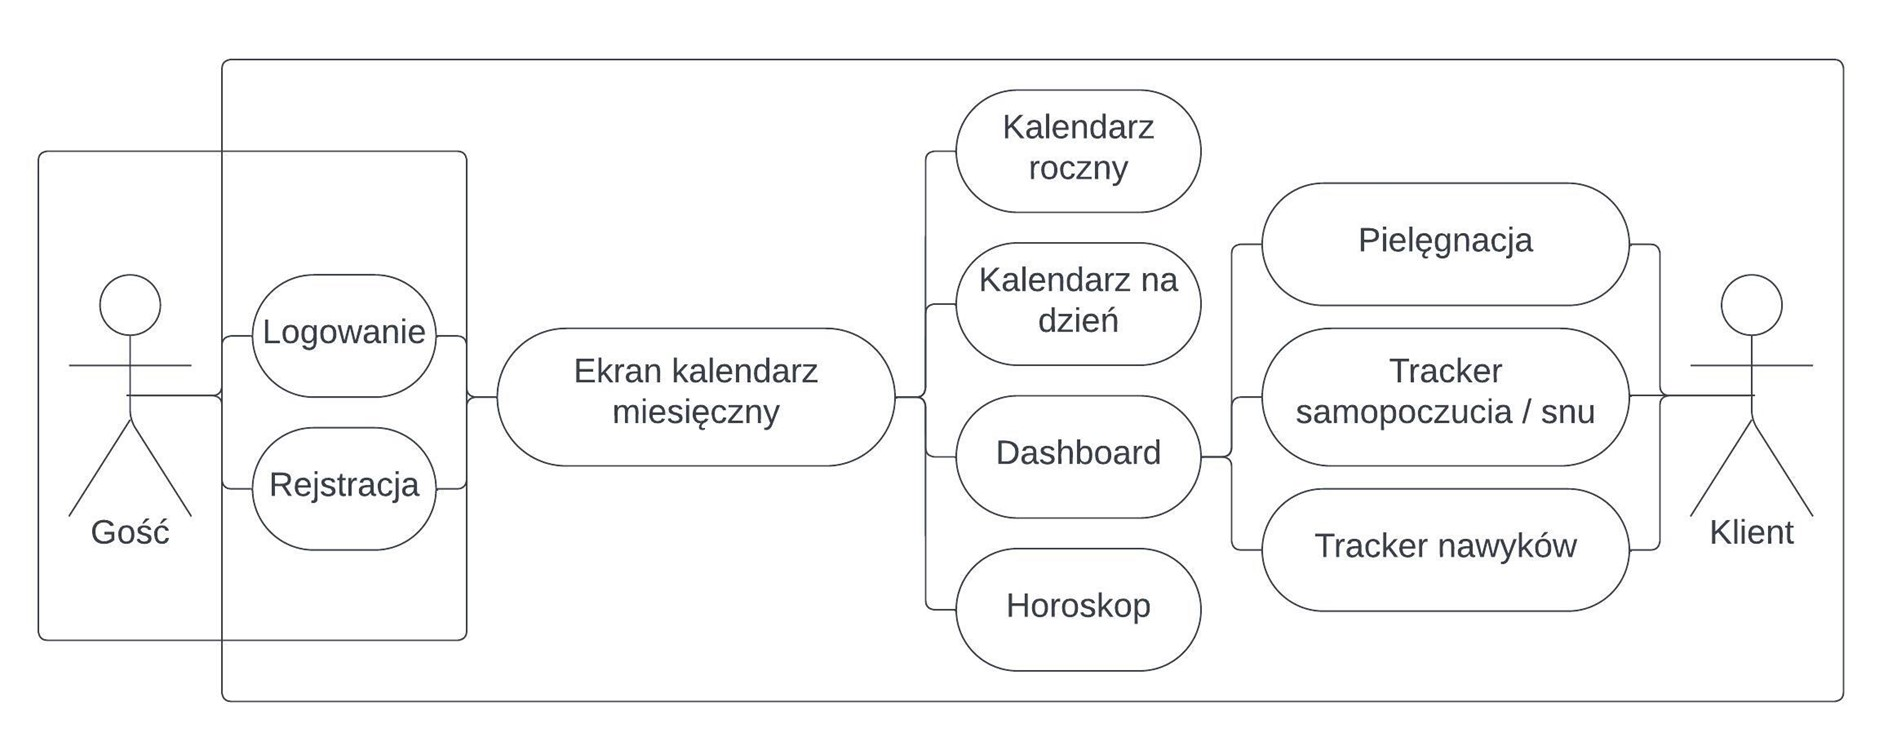
\includegraphics[width=1\linewidth]{images/model_danych/uml}
	\caption{Diagram UML komponentów}
	\label{fig:uml}
\end{figure}

NAPISAĆ CZYM SĄ KOMPONENTY!

\section{Diagram przypadków użycia}

SKOMPRESOWAĆ ODSTĘPY + NUMERKI ZAMIAST LITER W PODLIŚCIE! + WCIĘCIE PRZYPADEK UŻYCIA

\textbf{Przypadek użycia:} Rejestracja użytkownika

\textbf{Aktor:} Gość

\textbf{Opis:} Przypadek użycia "Rejestracja użytkownika" umożliwia nowym użytkownikom stworzenie konta w systemie. Rejestracja wymaga podania informacji, takich jak nazwę, adres e-mail, dzień urodzenia oraz hasło. Umożliwia to dostęp do pełnych funkcji systemu, takich jak logowanie, przeglądanie zawartości i zarządzanie swoim profilem.

\textbf{Warunki wstępne:} Gość odwiedza stronę rejestracji. Gość nie posiada konta w systemie.

\textbf{Przebieg:}

\begin{enumerate}
	\item Gość wchodzi na ekran rejestracji.
	\item System wyświetla formularz rejestracyjny.
	\item Gość wprowadza swoje dane, takie jak nazwę, adres e-mail, hasło oraz dzień urodzenia
	\item System sprawdza poprawność wprowadzonych danych.
	\begin{enumerate}
		\item Wprowadzone dane są poprawne.
		\begin{enumerate}
			\item Gość jest automatycznie zalogowany na nowo utworzone konto.
		\end{enumerate}
		\item Wprowadzone dane są niepoprawne.
		\begin{enumerate}
			\item Zostaje wyświetlony komunikat, że podane dane są niepoprawne. Użytkownik nie zostaje dodany do bazy danych.
		\end{enumerate}
	\end{enumerate}
\end{enumerate}


\textbf{Przypadek użycia:} Logowanie użytkownika

\textbf{Aktor:} Gość

\textbf{Opis:} Przypadek użycia "Logowanie użytkownika" umożliwia użytkownikom dostęp do
pełnych funkcji systemu. Logowanie wymaga podania informacji, takich jak adres e-mail
i hasło.

\textbf{Warunki wstępne:} Gość uruchamia aplikację. Użytkownik niezalogowany w serwisie.

\textbf{Przebieg:}


\textbf{Przypadek użycia:} Sprawdzenie horoskopu

\textbf{Aktor:} Klient

\textbf{Opis:} Przypadek użycia "Sprawdzenie horoskopu" umożliwia użytkownikom dostęp do
codziennych horoskopów dedykowany dla ich znaku zodiaku.

\textbf{Warunki wstępne:} Klient ma przydzielony znak zodiaku z bazy danych.

\textbf{Przebieg:}
\begin{enumerate}
	\item Klient przesuwa ekran w prawą stronę.
	\item Zostaje wyświetlona nazwa znaku zodiaku, ilustracja oraz horoskop na dany dzień.
\end{enumerate}
